\subsubsection{27.12.14}
\begin{enumerate}
	
	\item Time of beginning and ending of meeting: 16:15 - 20:00.
	
	\item Purposes of meeting: 
	\begin{enumerate}
		
		\item To finish soldering wires.
		
		\item To elaborate MCB that can to keep rolling goal when power off.
		
        \item To write more comfortable programme of control robot.
		
	\end{enumerate}

	\item Work that has been done:
	\begin{enumerate}
		
		\item All wires were soldered.
		
		\item It was decided to install on MCB two stickers so that MCB doesn't open due to weight of rolling goal when robot is on the ramp. Stickers were installed but didn't tested because we hasn't got original rolling goals.
		
		\begin{figure}[H]
			\begin{minipage}[h]{0.1\linewidth}
				\center  
			\end{minipage}
			\hfill
			\begin{minipage}[h]{0.29\linewidth}
				\center{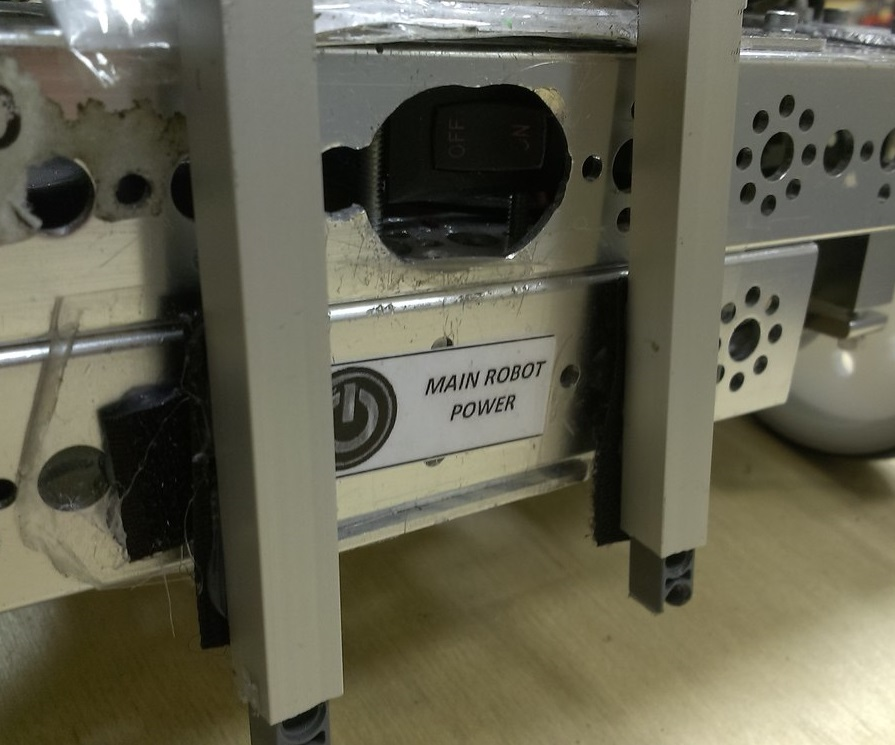
\includegraphics[scale=0.2]{days/27.12.14/images/01}}
			\end{minipage}
			\hfill
			\begin{minipage}[h]{0.29\linewidth}
				\center{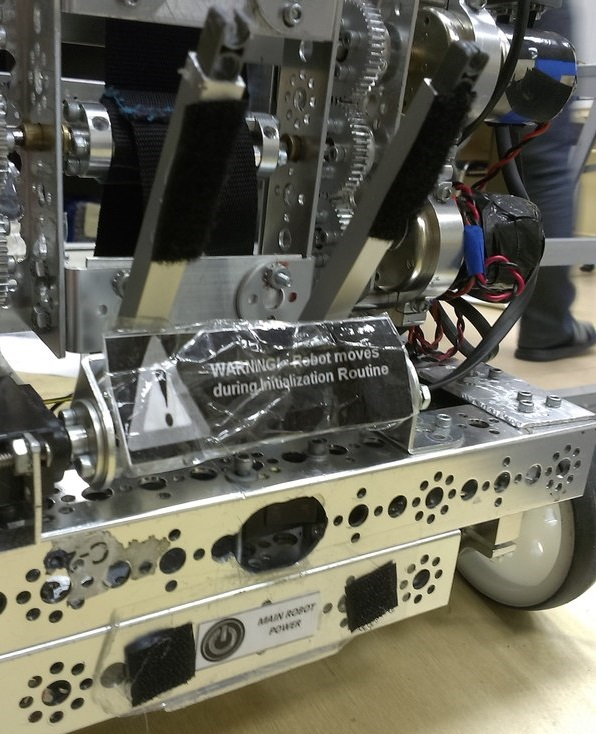
\includegraphics[scale=0.2]{days/27.12.14/images/02}}
			\end{minipage}
			\hfill
			\begin{minipage}[h]{0.1\linewidth}
				\center  
			\end{minipage}
			\caption{Stickers on MCB}
		\end{figure}
		
        \item It was wrote more comfortable programme of contorol robot. Now control of moving is by button "TopHat"8 ways: forward, backward, tank turning . Robot can move by   Была реализована более удобная программа управления движением робота. Управление движением с левого аналогового датчика (стика) было перенесено на многопозиционную кнопку "TopHat". Так, теперь можно задать роботу двигаться восемью способами: Вперед, назад, танковый разворот вокруг своей оси по часовой стрелке и против, а также вращение только одной парой приводов (левой или правой) вперед или назад, в результате чего получается разворот вокруг неподвижной пары приводов. Кроме того, при удержании кнопок 6 или 7 включается медленное движение.
		
        \begin{figure}[H]
	  	  \begin{minipage}[h]{0.2\linewidth}
	  		\center  
	  	  \end{minipage}
	  	  \begin{minipage}[h]{0.6\linewidth}
	  		\center{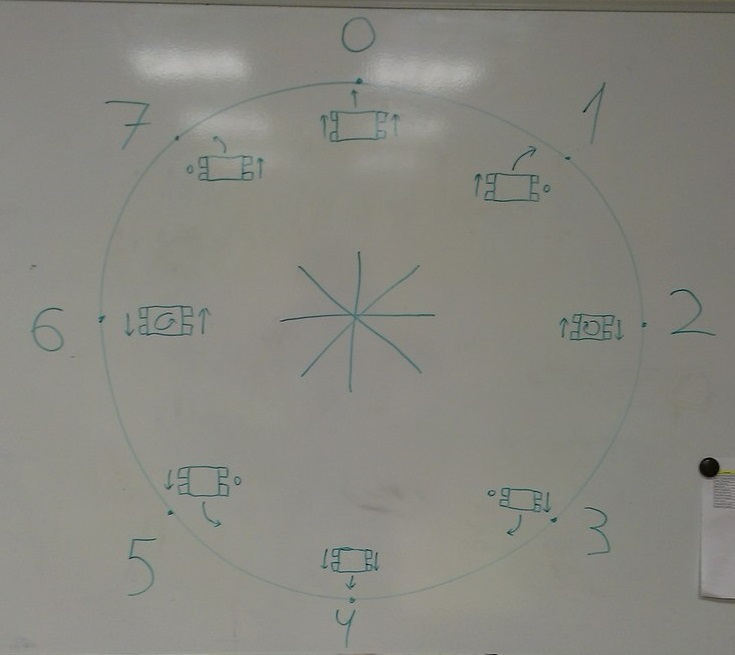
\includegraphics[scale=0.3]{days/27.12.14/images/03}}
	  		\caption{Схема управления движением}
	  	  \end{minipage}
	   \end{figure}
	   
	   \item Во время испытания программы движения было замечено, что замененный ранее привод (правый задний) не работает на поле (он прокручивается без нагрузки, когда робот находится на весу, но когда робот стоит на поле, этом привод не способен сдвинуть его с места). Несмотря на это, робот выполнял хорошо 5 из 8 команд (движение по прямой, разворот по часовой стрелке, развороты с использованием только левой парой колес). Опытным путем удалось выяснить, что неисправен именно привод, а не драйвер приводов. Необходимо снова заменить привод для того, чтобы робот мог нормально выполнять все возможные виды движения.
	   
	\end{enumerate}
	
	\item Results:
	\begin{enumerate}
		
		\item Все провода залужены.
		
		\item МЗК усовершенствован, но не испытан.
		
        \item Новая программа движения написана и протестирована. Результат положительный.
		
	\end{enumerate}
	
	\item Tasks for the next meetings:
	\begin{enumerate}
		
		\item Заменить сломанный привод.
		
		\item Заменить сломанную рейку подъемника.
			
	\end{enumerate}
\end{enumerate}
\fillpage
